\documentclass[14pt, fleqn, xcolor={dvipsnames, table}]{beamer}
\usepackage[T2A]{fontenc}
\usepackage[utf8]{inputenc}
\usepackage[english,russian]{babel}
\usepackage{amssymb,amsfonts,amsmath,mathtext}
\usepackage{cite,enumerate,float,indentfirst}
\usepackage{cancel}

\usepackage{tikz}                   
\usetikzlibrary{shadows}

% \usepackage{enumitem}
% \setitemize{label=\usebeamerfont*{itemize item}%
%   \usebeamercolor[fg]{itemize item}
%   \usebeamertemplate{itemize item}}

\graphicspath{{images/}}

\usetheme{Madrid}
\usecolortheme{seahorse}
\renewcommand{\CancelColor}{\color{red}}

\setbeamercolor{footline}{fg=Blue!50}
\setbeamertemplate{footline}{
  \leavevmode%
  \hbox{%
  \begin{beamercolorbox}[wd=.333333\paperwidth,ht=2.25ex,dp=1ex,center]{}%
    И. Кураленок, Н. Поваров, Яндекс
  \end{beamercolorbox}%
  \begin{beamercolorbox}[wd=.333333\paperwidth,ht=2.25ex,dp=1ex,center]{}%
    Санкт-Петербург, 2013
  \end{beamercolorbox}%
  \begin{beamercolorbox}[wd=.333333\paperwidth,ht=2.25ex,dp=1ex,right]{}%
  Стр. \insertframenumber{} из \inserttotalframenumber \hspace*{2ex}
  \end{beamercolorbox}}%
  \vskip0pt%
}
\newcommand\indentdisplays[1]{%
     \everydisplay{\addtolength\displayindent{#1}%
     \addtolength\displaywidth{-#1}}}
\newcommand{\itemi}{\item[\checkmark]}

\title{Линейные модели: введение\\\small{по материалам "The Elements of Statistical Learning"}}
\author[]{\small{%
И.~Куралёнок,
Н.~Поваров}}
\date{}

\begin{document}

\begin{frame}
\maketitle
\small
\begin{center}
\vspace{-60pt}
\normalsize {\color{red}Я}ндекс \\
\vspace{80pt}
\footnotesize СПб, 2013
\end{center}
\end{frame}

\section{Линейные модели}
\begin{frame}{Формальная постановка}
Ищем решающую функцию в виде:
$$
y = F(\lambda, x) = \lambda^T x
$$
Такое решение кажется примитивным!
\end{frame}
\begin{frame}{Формальная постановка}
Ищем решающую функцию в виде:
$$
y = F(\lambda, x) = \lambda^T x
$$
Такое решение кажется примитивным! \\
До того как мы расскажем что такое $x$.
\end{frame}
\begin{frame}{Какое $x$ бывает}
Просто фичи:
$$
x \in \mathbb{R}^n
$$
Мономы:
$$
u \in \mathbb{R}^n
x = \prod u_j
$$
Произвольные функции:
$$
u \in \mathbb{R}^n
x: \mathbb{R}^n \to \mathbb{R}
$$
В любом случае мы всегда можем посчитать значение $x$ по входным параметрам.
\end{frame}

\section{Линейная регрессия}
\begin{frame}{Простое решение}
$$
\arg \min_{\lambda} \|F(X, \lambda) - y\| = \arg \min_{\lambda} \|X \lambda - y\|
$$
Если норма $l_2$, то:
$$
{\partial T \over \partial X} = 2 X^T\left(X\lambda - y\right) = 0
$$
$$
\lambda_0 = (X^TX)^{-1}X^Ty
$$
\end{frame}

\begin{frame}{Геометрическая интерпретация}
\small
Если посмотреть на колонки, соответствующие фичам то картинка такая:
\begin{center}
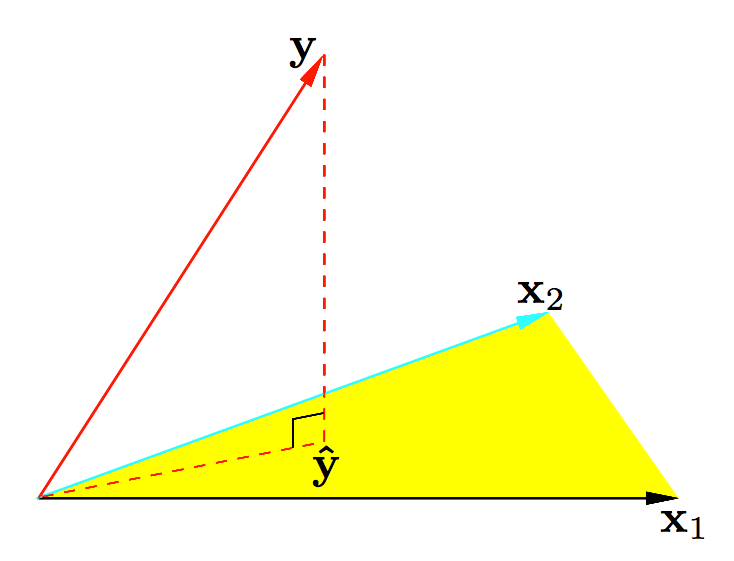
\includegraphics[height=0.4\textheight]{3_2.png}
\end{center}
Об этом говорит (если нам все удалось):
$$
X^T(y - \hat{y}) = X^T(y - X\lambda_0) = 0
$$
В случае, если $rank(X) < n$ ортогональность остается!
\end{frame}

\subsection{Статистические свойства решения}
\begin{frame}{Статистические свойства решения}
Если наблюдения независимы, $Var(y) = const$, а $x$ вычислены точно:
$$
Var(\lambda) = \left(X^TX\right)^{-1}\frac{1}{m - n - 1}\|y - \hat{y}\|_2
$$
А если еще и предположить, что $y=\lambda_1^Tx + \epsilon$ и $\epsilon \sim N(0,\sigma)$:
$$
\lambda_0 \sim N(\lambda_1, \left(X^TX\right)^{-1}\sigma^2)
$$
а наблюдаемая $\sigma$ для $y$ распределена по $\chi^2$:
$$
(n-m-1)\hat{\sigma} = \|y - \hat{y}\|_2 \sim \sigma \chi^2_{m-n-1}
$$
\end{frame}

\begin{frame}{А точно $\lambda_{0_i} \ne 0$?}
Введем такую штуку ($Z$-score):
$$
z_i = \frac{\lambda_{0_i}}{\hat{\sigma}\sqrt{v_i}}
$$
где $v_i$ --- диагональный элемент $\left(X^TX\right)^{-1}$. Если подумать что $\lambda_{0_i} = 0$, то:
$$
z_i \sim T_{m-n-1}
$$
Чем больше $Z$-score, тем более мы уверены, что $\lambda_{0_i} \ne 0$
\end{frame}

\subsection{Теорема Гаусса-Маркова}
\begin{frame}{Теорема Гаусса-Маркова}
\begin{theorem}[]
Линейное приближение по MSE обладает на наименьшим разбросом из всех несмещенных линейных решений
\end{theorem}
\begin{itemize}
\item[$\Rightarrow$] для того, чтобы сделать решение более стабильным надо вводить bias
\item[$\Rightarrow$] простым MSE нам не отделаться, надо будет менять $T$
\end{itemize}
\end{frame}

\subsection{Расширение на несколько целевых функций}
\begin{frame}{Расширение на несколько целей}
$$
y_i \in \mathbb{R}^k
$$
В этом случае задача превращается в такую:
$$
\arg \min_\Lambda tr\left((Y - X\Lambda)^T(Y - X\Lambda)\right)
$$
$$
\Lambda_0 = \left(X^TX\right)^{-1} X^TY
$$
Если же $y = x^T\Lambda + \epsilon$, $\epsilon \sim N(0, \Sigma)$:
$$
\arg \min_\Lambda \left((Y - X\Lambda)^T\Sigma^{-1}(Y - X\Lambda)\right)
$$
\end{frame}

\section{Линейная классификация}
\begin{frame}{Классификация}
$$
x \in \mathbb{R}^n, y \in \{1,\ldots, k\}
$$
\begin{center}
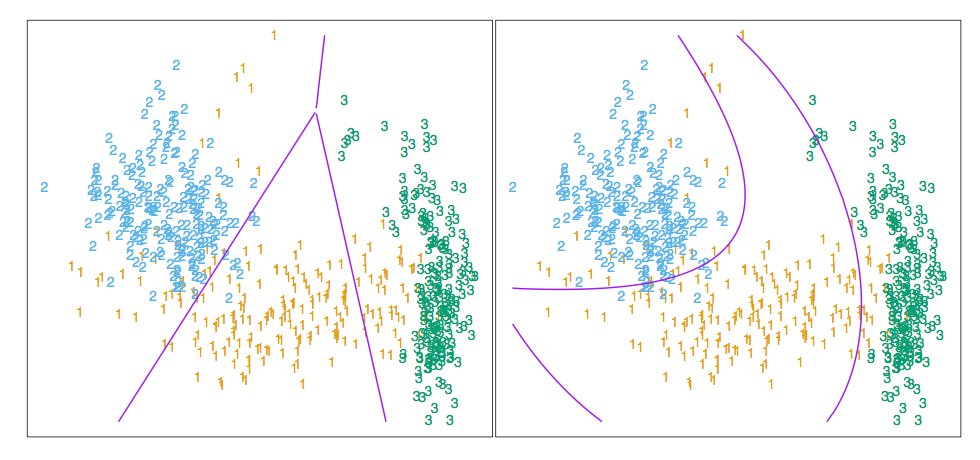
\includegraphics[height=0.4\textheight]{4_1.png}
\end{center}
\small
Введем дискриминационные функции для каждого класса. У какого класса больше, тот и молодец. Там где равны --- границы решения.\\
NB: монотонные преобразования дискриминационным функциям не страшны
\end{frame}

\subsection{Простая линейная модель и ее вариации}
\begin{frame}{Линейное решение задачи классификации}
Можем пойти по-простому и решить регрессией:
$$
\gamma_{ij} = \left\{\begin{array}{ll}
1,& i = y_i \\
0 
\end{array}\right.
$$
В терминах предсказания $\gamma$ решаем:
$$
\arg \min_\Lambda tr\left((\Gamma - X\Lambda)^T(\Gamma - X\Lambda)\right)
$$
\end{frame}

\begin{frame}{Сложности с простым решением}\small
\begin{center}
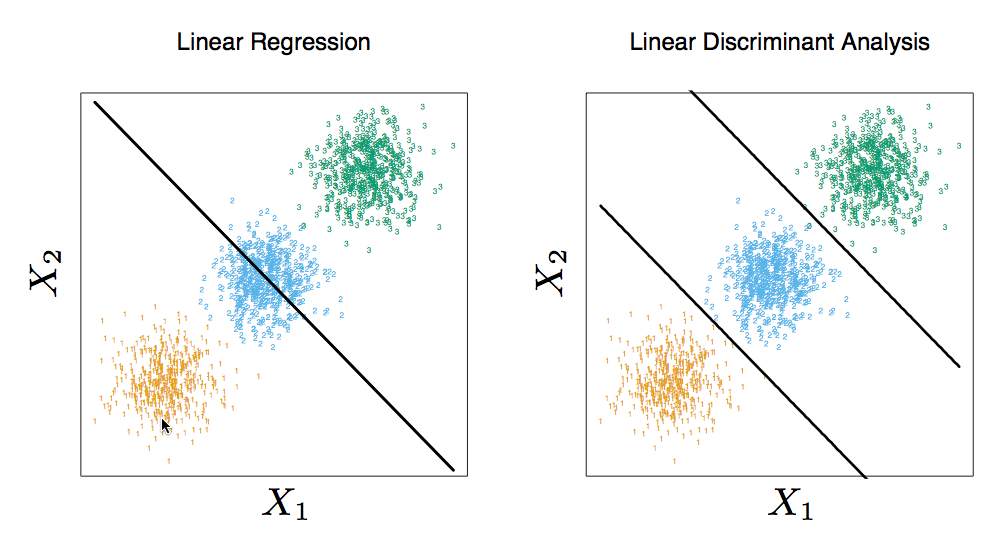
\includegraphics[width=0.8\textwidth]{4_2.png}
\end{center}
\end{frame}

\subsection{Линейный дискриминантный анализ (LDA)}
\begin{frame}{Линейный дискриминантный анализ (LDA)}
Представим себе, что точки порождены смесью нормальных распределений по одному на класс:
$$
f_j = \frac{1}{\sqrt{(2\pi)^n|\Sigma_j|}}e^{-\frac{1}{2}(x - \mu_j)^T\Sigma^{-1}_j(x - \mu_j)}
$$
Границы решения прямые! Если зафиксировать $\Sigma$:
$$
f_j(x) = x^T\Sigma^{-1}\mu_j - \frac{1}{2}\mu_j^T\Sigma^{-1}\mu_j + log \pi_j
$$
\end{frame}
\begin{frame}{LDA: решение}
Можно решать напрямую:
$$\begin{array}{c}
\pi_j = \frac{m_j}{m},\\
\mu_j = \frac{1}{m_j}\sum_{x_u:y_u = j} x_u,\\
\Sigma = \frac{1}{m-k}\sum_{j=1}^k\sum_{x_u:y_u = j}(x_u - \mu_j)(x_u - \mu_j)^T \\
\end{array}$$
Можно $EM$ даже не заморачиваясь одинаковыми $\Sigma_j$
\end{frame}
\begin{frame}{LDA: свойства}
\begin{itemize}
  \item Нормальные распределения в основе
  \item Решение в аналитическом виде
  \item Работает даже в далеких от ``гауссовых'' ситуаций
  \item Имеет расширение в квадратичные мономы (QDA)
  \item Часто рассматривают диагональные $\Sigma_k$ для ускорения вычислений
  \item Можно использовать $\Sigma_k = \alpha\Sigma_0 + (1 - \alpha)\Sigma^k$
\end{itemize}
\end{frame}

\subsection{Логистическая регрессия}

\begin{frame}{Логистическая регрессия}
Будем искать не дискриминантные функции, а напрямую границы между классами:
$$
log\left(\frac{P(y=u|x)}{P(y=k|x)}\right) = x^T \lambda_{u}
$$
Преобразование справа --- logit. Тогда вероятности можно найти так:
$$
p(y=u|x) = {x^T \lambda_{u} \over 1 + \sum_{v < k} x^T\lambda_v}, u < k
$$
$$
p(y=k|x) = {1 \over 1 + \sum_{v < k} x^T\lambda_v}
$$
\end{frame}

\begin{frame}{Оптимизация логистическая регрессия}
Вероятности у нас есть, давайте максимизировать правдоподобие!
$$
\arg \max_\Lambda \prod_i p(y_i|x_i, \Lambda)
$$
$$
= \arg \max_\Lambda \sum_i log {x^T \lambda_{u} \over 1 + \sum_{v < k} x^T\lambda_v}
$$
Как будем искать?
\end{frame}

\begin{frame}{Оптимизация логистическая регрессия}
Вероятности у нас есть, давайте максимизировать правдоподобие!
$$
\arg \max_\Lambda \prod_i p(y_i|x_i, \Lambda)
$$
$$
= \arg \max_\Lambda \sum_i log {x^T \lambda_{u} \over 1 + \sum_{v < k} x^T\lambda_v}
$$
Как будем искать?
\end{frame}

\begin{frame}{Когда что?}
\begin{itemize}
  \item Есть много точек, для которых нет оценок $\Rightarrow$ LDA
  \item Есть подозрение на близость к норамльности $\Rightarrow$ LDA
  \item Хотим использовать prior $\Rightarrow$ LDA
  \item Во всех остальных случаях логистическая регрессия, особенно если есть много outlier'ов
\end{itemize}
\end{frame}

\section{Бонус: метрики классификации}

\section{Домашнее задание}
\begin{frame}{Результаты ДЗ второй недели}
\scriptsize
\begin{center}
\begin{enumerate}
\item 6af9df
\item dccc3e
\item f33f66
\item f1015e
\item f33f2d
\item 458048
\item 93184e
\item 608072
\item 824e76
\item 88d593
\item cfd271
\item 48364c
\item c5b930
\item 080c07
\item 579569
\item 01b988
\item 68c819
\item dcb652
\item ba605a
\item 692f0b
\item 6aca1b
\end{enumerate}
%Не отличаются 1-2 место, 3-6, 8-15, 16-21
\end{center}
\end{frame}
\begin{frame}{Домашнее задание}
\begin{itemize}
\item SVN, howto.txt
\item Две недели
\end{itemize}
\end{frame}
\end{document}
